\section{Arquitectura Kappa}

\subsection{Principios de Diseño}

La principal característica de esta arquitectura es su fuerte uso de un registro de eventos inmutable 
y ordenado cronológicamente que actúa como única fuente de verdad sobre los datos ingresados al sistema.

De esta manera, se logra unificar el procesamiento de datos en batch y streaming tratándolos como un flujo continuo de eventos, 
eliminando la dualidad de código y reduciendo la complejidad operativa.

El procesamiento de estos datos se realiza mediante motores de procesamiento de eventos que leen este registro, 
aplican transformaciones determinísticas 
y generan resultados derivados que pueden recomputarse en cualquier momento desde el inicio del log.

Este principio de reproducibilidad permite regenerar el estado completo del sistema cuando cambian los requisitos 
o algoritmos de procesamiento, sin necesidad de mantener rutas de código separadas.

Las vistas materializadas son otro principio fundamental, 
donde los resultados procesados se almacenan en sistemas optimizados para consultas, 
proporcionando acceso eficiente al estado actual sin necesidad de reprocesar todo el historial de eventos.

\newpage
\subsection{Stack Tecnológico}

Para la capa de ingesta y transporte de datos, la Arquitectura Kappa implementa \textbf{Apache Kafka} como componente central, 
funcionando no solo como sistema de mensajería sino como la fuente única de verdad y almacén principal de eventos. 
En Kappa se configura Kafka con períodos de retención extendidos, 
aprovechando la capacidad de compactación de logs para mantener el historial completo de eventos mientras 
se optimiza el espacio de almacenamiento. 
Esto se logra agregando la capacidad de almacenamiento en capas, mediante la cual se pueden mantener los eventos
en Object Storage (utilizando \textbf{MinIO}), cuando pasa un tiempo definido de mantención en almacenamiento local.

El procesamiento de datos se realiza mediante \textbf{Apache Flink},
se despliega en un cluster con un nodo Job Manager y cuatro nodos Task Manager; de forma de distribuir la carga de trabajo lo mejor posible.
En este caso, se define como punto de entrada un tópico de Kafka, para procesar los datos en tiempo real y
enviarlos a un nuevo topico y continuar con el procesamiento más adelante en la arquitectura.

En el último paso, se guarda el resultado del procesamiento en \textbf{Apache Doris}, un motor de análisis de datos
distribuido que permite realizar consultas SQL en tiempo real sobre grandes volúmenes de datos con una interfaz basada en MySQL.
Este componente permite escalar de forma diferente el acceso a los datos del procesamiento, 
siendo desplegado como un nodo frontend y tres nodos backend. 
Estos comparten el trabajo de procesamiento de consultas y almacenamiento de datos, 
mientras que el frontend se encarga de la distribución de las mismas. 

\newpage
\subsection{Vista de Componentes}

\begin{figure}[h]
    \makebox[\textwidth]{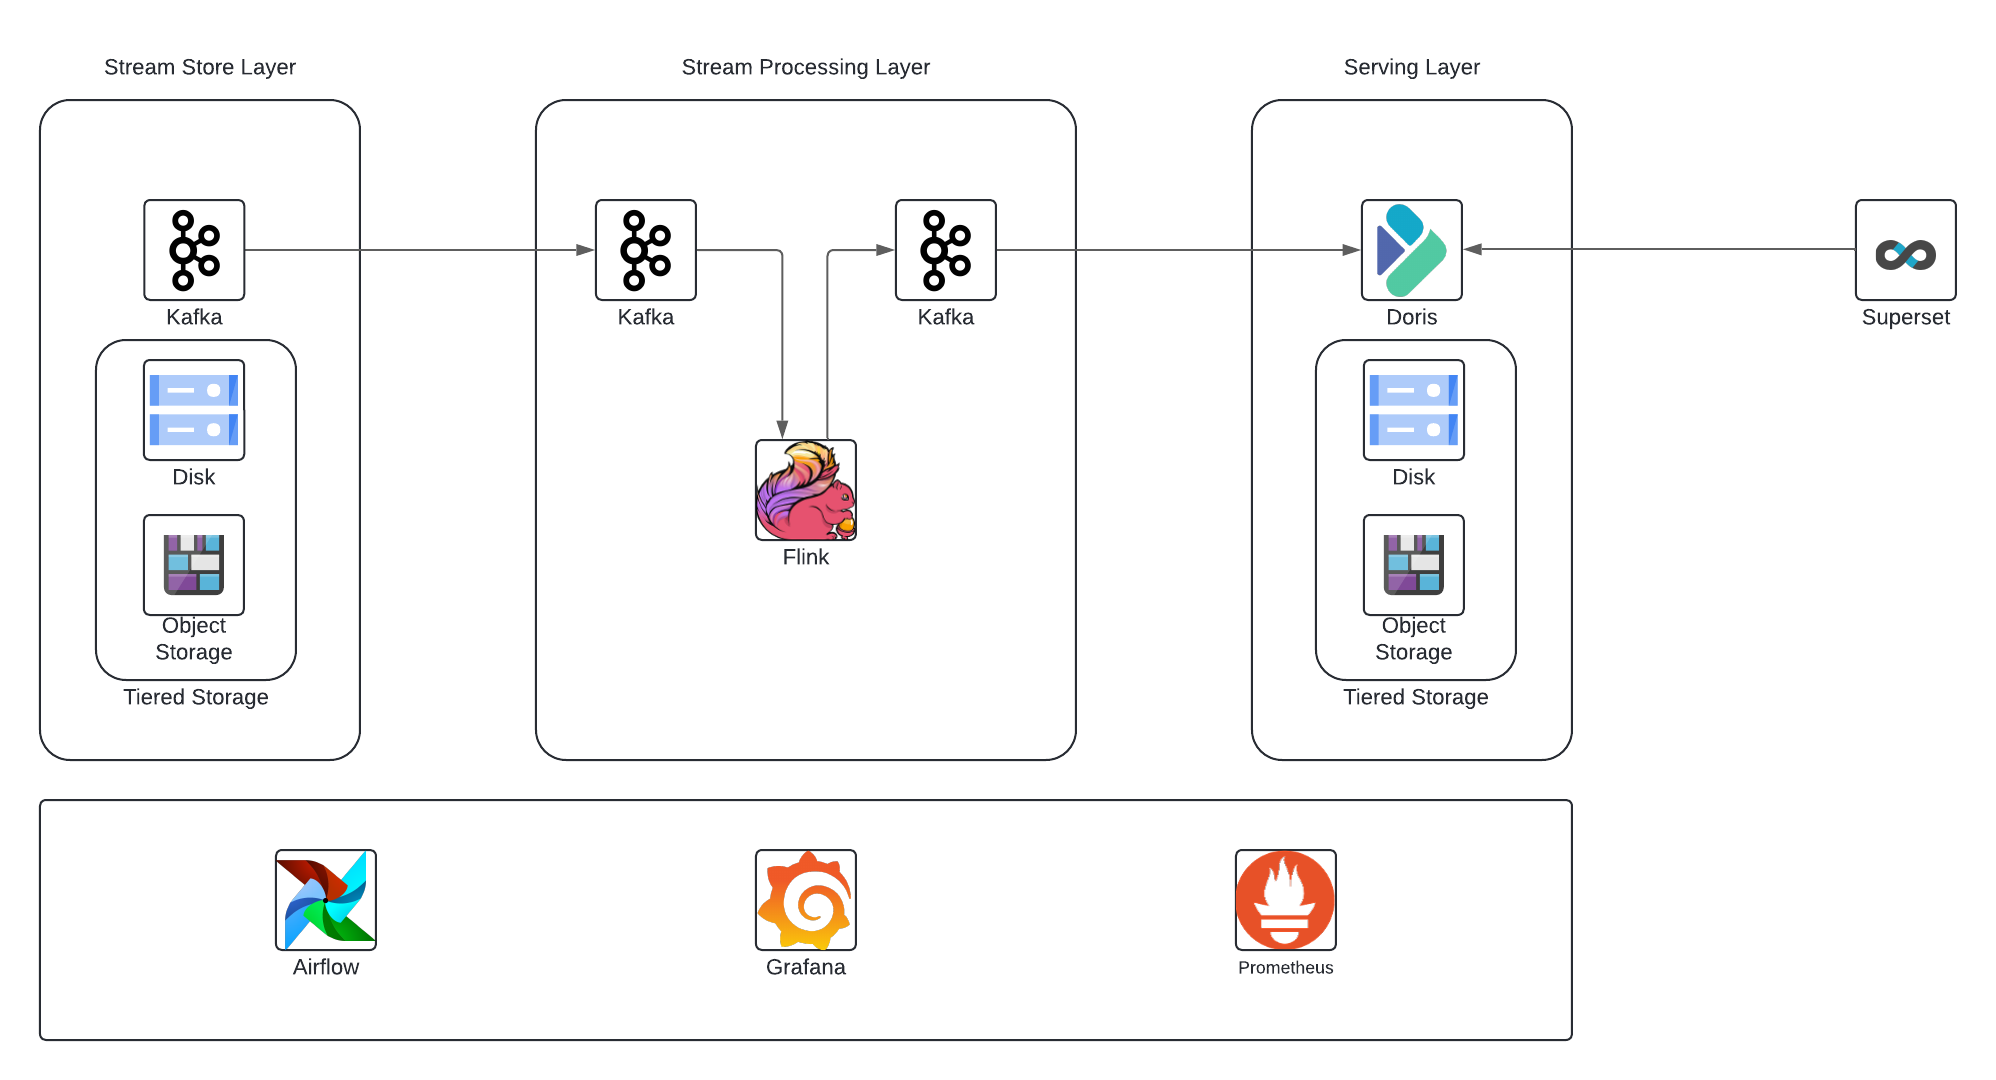
\includegraphics[width=\paperwidth]{desarrollo/Kappa.png}}
    \caption{Diagrama de la Arquitectura Kappa}
    \label{fig:des_arquitectura_kappa}
\end{figure}

\newpage

\subsection{Flujo de Procesamiento}

El siguiente es un ejemplo de uno de los trabajos de procesamiento de datos desarrollados:

\begin{lstlisting}[language=sql]
    SET 'execution.runtime-mode' = 'streaming';
    SET 'execution.checkpointing.mode' = 'EXACTLY_ONCE';
    SET 'table.local-time-zone' = 'UTC';
    SET 'execution.checkpointing.interval' = '60000';
    SET 'execution.checkpointing.timeout' = '30000';
    SET 'state.backend' = 'hashmap';
    SET 'table.exec.state.ttl' = '300000';
    SET 'parallelism.default' = '4';
\end{lstlisting}

\begin{lstlisting}[language=sql]
    -- Raw measurements table with original timestamps and device metrics
    CREATE TABLE raw_measurements (
        measurement_timestamp TIMESTAMP(3),
        measurement_type STRING,
        raw_value STRING,
        device_id STRING,
        battery DOUBLE,
        signal_strength DOUBLE,
        ingestion_timestamp TIMESTAMP(3) METADATA FROM 'timestamp' VIRTUAL,
        WATERMARK FOR measurement_timestamp AS measurement_timestamp - INTERVAL '10' SECONDS
    ) WITH (
        'topic' = 'raw.measurements',
        'connector' = 'kafka',
        'properties.bootstrap.servers' = 'kafka-1:19091,kafka-2:19092,kafka-3:19093',
        'format' = 'json',
        'json.timestamp-format.standard' = 'ISO-8601',
        'scan.startup.mode' = 'latest-offset'
    );
\end{lstlisting}
\newpage
\begin{lstlisting}[language=sql]
    CREATE TABLE enriched_measurements (
        measurement_type STRING,
        `value` DOUBLE,
        device_id STRING,
        patient_id STRING,
        
        -- Weights
        quality_weight DOUBLE,
        freshness_weight DOUBLE,
        
        -- Timestamps
        measurement_timestamp TIMESTAMP(3),
        ingestion_timestamp TIMESTAMP(3),
        enrichment_timestamp TIMESTAMP(3) METADATA FROM 'timestamp' VIRTUAL,
        WATERMARK FOR measurement_timestamp AS measurement_timestamp - INTERVAL '10' SECONDS
    ) WITH (
        'topic' = 'enriched.measurements',
        'connector' = 'kafka',
        'properties.bootstrap.servers' = 'kafka-1:19091,kafka-2:19092,kafka-3:19093',
        'format' = 'json',
        'json.timestamp-format.standard' = 'ISO-8601',
        'scan.startup.mode' = 'latest-offset'
    );
\end{lstlisting}
\newpage
\begin{lstlisting}[language=sql]
    -- Insert with quality and freshness calculations
    INSERT INTO enriched_measurements
    SELECT
        measurement_type,
        CAST(raw_value AS DOUBLE) AS `value`,
        device_id,
        REGEXP_EXTRACT(device_id, '.*_(P\d+)$', 1) AS patient_id,

        -- Quality components
        CAST((
            CASE
                WHEN device_id LIKE 'MEDICAL%' THEN 1.0
                WHEN device_id LIKE 'PREMIUM%' THEN 0.7
                ELSE 0.4
            END * 0.7 +
            CASE
                WHEN battery >= 80 THEN 1.0
                WHEN battery >= 50 THEN 0.8
                WHEN battery >= 20 THEN 0.6
                ELSE 0.4
            END * 0.2 +
            CASE
                WHEN signal_strength >= 0.8 THEN 1.0
                WHEN signal_strength >= 0.6 THEN 0.8
                WHEN signal_strength >= 0.4 THEN 0.6
                ELSE 0.4
            END * 0.1
        ) AS DECIMAL(7,2)) AS quality_weight,

        -- Combined freshness calculation
        CASE
            WHEN TIMESTAMPDIFF(HOUR, measurement_timestamp, ingestion_timestamp) <= 1 THEN 1.0
            WHEN TIMESTAMPDIFF(HOUR, measurement_timestamp, ingestion_timestamp) <= 6 THEN 0.9
            WHEN TIMESTAMPDIFF(HOUR, measurement_timestamp, ingestion_timestamp) <= 12 THEN 0.7
            WHEN TIMESTAMPDIFF(HOUR, measurement_timestamp, ingestion_timestamp) <= 24 THEN 0.5
            WHEN TIMESTAMPDIFF(HOUR, measurement_timestamp, ingestion_timestamp) <= 48 THEN 0.3
            ELSE 0.2
        END AS freshness_weight,
        
        -- Timestamps
        measurement_timestamp,
        ingestion_timestamp
    FROM raw_measurements;
\end{lstlisting}

Como se puede ver, FLink SQL permite tratar a los tópicos de Kafka como tablas, pudiendose así leer y escribir sobre ellos. 
Esto permite realizar un procesamiento de datos en tiempo real,
enriquecerlos y enviarlos a otro tópico de Kafka para su posterior procesamiento.

Para esta arquitectura se utilizaron dos conectores diferentes de Kafka. El primero, visto en los ejemplos, permite leer y escribir pero no modificar. 
Por otro lado, para las agregaciones, se utilizó \textbf{upsert-kafka} que agrega la semántica de actualización y borrado de mensajes,
que es muy útil para cuando se necesita un procesamiento incremental de la información, como es el caso de las agregaciones. 
Aunque cabe destacar que la potencia de Flink permite que se pueda hacer esto incluso para otros destinos de datos como se verá más adelante para Paimon.
Todo esto sin cambiar el código del trabajo de procesamiento. 

\newpage

\begin{lstlisting}[language=sql]
    CREATE TABLE scores (
        patient_id STRING,
        window_start TIMESTAMP(3),
        window_end TIMESTAMP(3),

        respiratory_rate_value DOUBLE,
        oxygen_saturation_value DOUBLE,
        blood_pressure_value DOUBLE,
        heart_rate_value DOUBLE,
        temperature_value DOUBLE,
        consciousness_value DOUBLE,

        respiratory_rate_score DOUBLE,
        oxygen_saturation_score DOUBLE,
        blood_pressure_score DOUBLE,
        heart_rate_score DOUBLE,
        temperature_score DOUBLE,
        consciousness_score DOUBLE,

        respiratory_rate_trust_score DOUBLE,
        oxygen_saturation_trust_score DOUBLE,
        blood_pressure_trust_score DOUBLE,
        heart_rate_trust_score DOUBLE,
        temperature_trust_score DOUBLE,
        consciousness_trust_score DOUBLE,

        measurement_timestamp TIMESTAMP(3),
        ingestion_timestamp TIMESTAMP(3),
        enrichment_timestamp TIMESTAMP(3),
        routing_timestamp TIMESTAMP(3),
        scoring_timestamp TIMESTAMP(3),
        union_timestamp TIMESTAMP(3),
        WATERMARK FOR union_timestamp AS union_timestamp - INTERVAL '10' SECONDS,
        PRIMARY KEY (patient_id, window_start) NOT ENFORCED
    ) WITH (
        'connector' = 'upsert-kafka',
        'topic' = 'scores',
        'properties.bootstrap.servers' = 'kafka-1:19091,kafka-2:19092,kafka-3:19093',
        'key.format' = 'json',
        'value.format' = 'json'
    );
\end{lstlisting}

\newpage

\begin{lstlisting}[language=sql]
    INSERT INTO scores
    SELECT * FROM (
        WITH unions as (
            ...
        )
        SELECT 
            patient_id,
            window_start,
            MAX(window_end) as window_end,

            MAX(CASE WHEN measurement_type = 'RESPIRATORY_RATE' THEN `value` END) as respiratory_rate_value,
            MAX(CASE WHEN measurement_type = 'OXYGEN_SATURATION' THEN `value` END) as oxygen_saturation_value,
            MAX(CASE WHEN measurement_type = 'BLOOD_PRESSURE_SYSTOLIC' THEN `value` END) as blood_pressure_value,
            MAX(CASE WHEN measurement_type = 'HEART_RATE' THEN `value` END) as heart_rate_value,
            MAX(CASE WHEN measurement_type = 'TEMPERATURE' THEN `value` END) as temperature_value,
            MAX(CASE WHEN measurement_type = 'CONSCIOUSNESS' THEN `value` END) as consciousness_value,

            ...

            MIN(measurement_timestamp) AS measurement_timestamp,
            MIN(ingestion_timestamp) AS ingestion_timestamp,
            MIN(enrichment_timestamp) AS enrichment_timestamp,
            MIN(routing_timestamp) AS routing_timestamp,
            MIN(scoring_timestamp) AS scoring_timestamp,
            CURRENT_TIMESTAMP as union_timestamp
        FROM TABLE(
            TUMBLE(
                TABLE unions, 
                DESCRIPTOR(measurement_timestamp), 
                INTERVAL '1' MINUTES
            )
        ) AS unions 
        GROUP BY patient_id, window_start
    ) as t;
\end{lstlisting}

\newpage
Por último, se guarda el resultado del procesamiento en \textbf{Apache Doris} directamente desde Flink.
Para esto, es necesario que la tabla en Doris haya sido creada previamente y además definir un nombre con el que llamarla en el trabajo de procesamiento.
Luego, se puede insertar los datos y Flink y Doris acordarán la forma de hacerlo. Según las pruebas realizadas, esto se hace en batches. 
El tiempo, entre que se terminó de procesar y fue insertado en Doris no fué posible de medir ya que no se encontraró una forma de definir la fecha de inserción real.

\newpage

\begin{lstlisting}[language=SQL]
    CREATE TABLE doris_gdnews2_scores (
        patient_id STRING,
        window_start TIMESTAMP(3),
        window_end TIMESTAMP(3),

        -- AVG Raw measurements
        ...

        -- Raw NEWS2 scores
        ...
        news2_score DOUBLE,

        -- Trust gdNEWS2 scores
        ...

        news2_trust_score DOUBLE,

        -- Timestamps
        measurement_timestamp TIMESTAMP(3),
        ingestion_timestamp TIMESTAMP(3),
        enrichment_timestamp TIMESTAMP(3),
        routing_timestamp TIMESTAMP(3),
        scoring_timestamp TIMESTAMP(3),

        flink_timestamp TIMESTAMP(3),
        aggregation_timestamp TIMESTAMP(3),
        PRIMARY KEY (patient_id, window_start) NOT ENFORCED
    ) WITH (
        'connector' = 'doris',
        'fenodes' = '172.20.4.2:8030',
        'table.identifier' = 'kappa.gdnews2_scores',
        'username' = 'kappa',
        'password' = 'kappa',
        'sink.label-prefix' = 'doris_sink_gdnews2',
        'sink.properties.format' = 'json',
        'sink.properties.timezone' = 'UTC'
    );
\end{lstlisting}

\begin{lstlisting}[language=SQL]
    INSERT INTO doris_gdnews2_scores
    SELECT *
    FROM gdnews2_scores;
\end{lstlisting}